\section{Stream Processing Architecture}\label{sec:concepts}
% Describe different ideas for distribution of events on multiple threads/processing and machines.  
We have designed a data stream processing pipeline architecture based on event producers and consumers concept which can be used to distribute
the processing tasks to multiple threads (on a single machine), multiple processes (distribution on many commodity machines), or a combination of both. 
Figure \ref{fig:parallel-srream-processing1} depicts our system architecture. The producers read the data stream batches from the remote 
network API (provided by debs2022 challenge \cite{debs2022challenge}), and store them in a buffer queue in main memory. 
The buffer queue has a specific size limitation that can be configured based 
on the available machine's RAM. The producer will read the data batches and stored them in the queue until the queue size reaches a specific limit, then 
go to sleep mode until the queue size is under another lower-level limit, and then wake up to producer data. 

The processing consumers access the batch from the queue and process the events for query 1 (values of $EMA_{38}$ and $EMA_{100}$) 
and the subsequent query 2. For the computation of $EMAs$ each consumer requires to know about the last $EMA$ value of the previous batch for a given stock symbol. 
The consumers are our main query processing units that we call consumers for for the sake of simplicity in this paper. 

\begin{figure*}[!ht]
    \begin{center}
        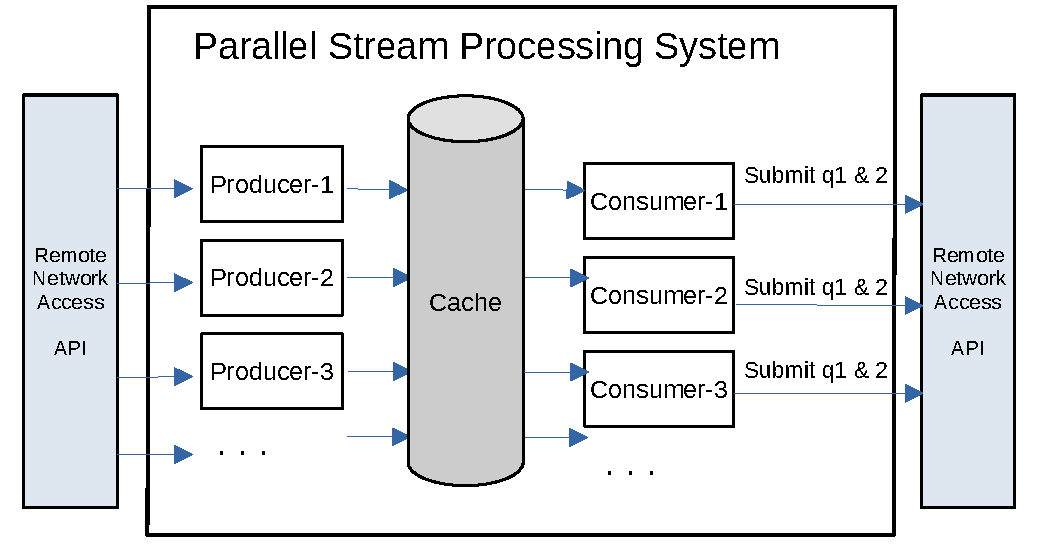
\includegraphics[width=0.7\textwidth]{./images/Parallel-Stream-Processing-System_v1}
        \caption{Parallel Processing of Events By a Set of Producers and Consumers without a Data Dispatcher.}
        \label{fig:parallel-srream-processing1}
    \end{center}
\end{figure*}


To make sure that there is no single bottleneck and synchronization lock point in this processing architecture, we made each of the consumers
(processing units) to be responsible for monitoring and computation of a sub-set of stocks symbol. Each consumer accesses the stream batches from 
the main memory cache and process only those that this consumer is responsible for. This can be implemented by using hash functions on 
stock symbol and mapping it to the id number of the consumer. 

Each consumer has a hash table that it uses to memorize the previous values of moving averages for different stock symbols.  
Each consumer has to access parts of each batch, and compute those stock symbols that this consumer is responsible for. In this way, each consumer can work 
independent of any other consumers in a functional form. The access to each data batch from the queue should be implemented in an efficient way so that each 
consumer does not read the entire batch to filter out the stock symbols. 



Figures \ref{fig:parallel-srream-processing} and \ref{fig:batch-distributions} illustrate how the system design would be if we have included an event dispatcher
and an event submitter. We do not have a dispatcher and submitter because of efficiency reasons and because of correctness of query processing. 
If we dispatch the event batches as shown in Figure \ref{fig:parallel-srream-processing}, for example by round-robin batch distribution, then each 
consumer has to work on all stock symbols or on a subset of them. If consumer work on all of the stocks, then each consumer requires to know the previous 
moving averages from the immediate past batch to compute the new EMAs for this batch, and this would cause incorrect processing because 
consumer should work in parallel distributed design without any dependencies on each other's results. In the latter case, if the consumers 
work on a subset of stocks then we need to pass every single batch to all of them and it is better 
to this task in an integrated form with reading from the queue.



\begin{figure*}[]
    \begin{center}
        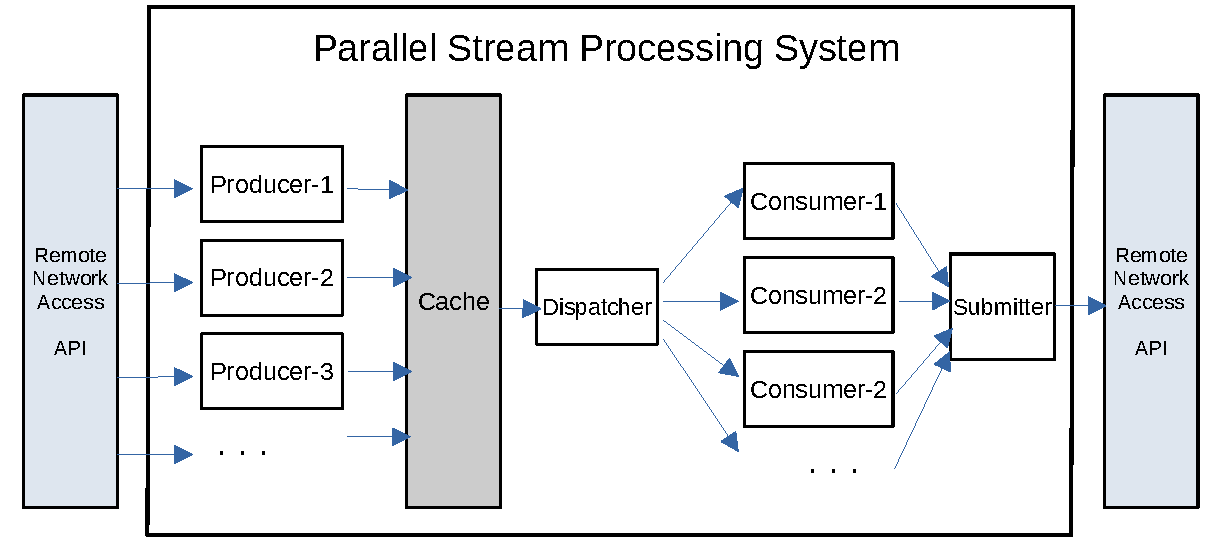
\includegraphics[width=0.7\textwidth]{./images/Parallel-Stream-Processing-System}
        \caption{Avoid Having a Event Dispatcher and Submitter.}
        \label{fig:parallel-srream-processing}
    \end{center}
\end{figure*}


\begin{figure*}[]
    \begin{center}
        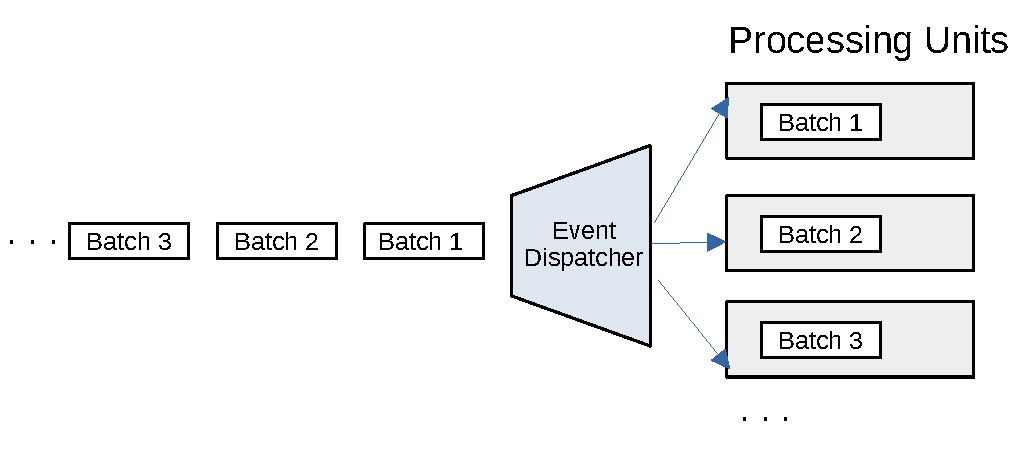
\includegraphics[width=0.7\textwidth]{./images/Stream-Batch-Distributions}
        \caption{An Event Data Dispatcher (Avoiding having a Dispatcher)}
        \label{fig:batch-distributions}
    \end{center}
\end{figure*}

Figure \ref{fig:Sequential-batch-distributions} illustrates how a sequential data stream processing can work to process the batches in multiple 
serial event consumers (processing units). Each processing unit will pick up and process a subset of stock market events. 
In a single machine setup the overhead of passing the event batches to the next consumer is very small but in a distributed setting the 
overhead of passing data batches to the next consumer over the network is very high because of data serialization costs. Comparing the 
architecture of Figure \ref{fig:Sequential-batch-distributions} and \ref{fig:parallel-srream-processing}, we preferred to implement the system 
parallel format shown in Figure \ref{fig:parallel-srream-processing}. 

\begin{figure*}[]
    \begin{center}
        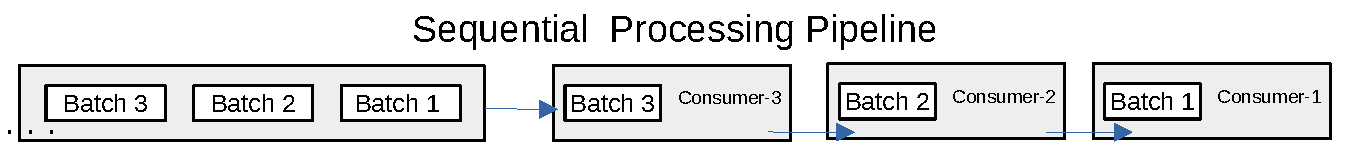
\includegraphics[width=0.7\textwidth]{./images/Stream-Batch-Distributions_op2}
        \caption{A Sequential Processing Pipeline. Each consumer reads a batch and passes to the next consumer. }
        \label{fig:Sequential-batch-distributions}
    \end{center}
\end{figure*}

The stream processing system will terminate if the stream of data is terminated, producers can not generate more event batches 
and there is no event batch in the buffer queue. 


%%%%%%%%%%%%%%%%%%%%%%%%%%%%%%%%%%%%%%%%%%%%%%%%%%%%%%%%
%%%%%%%%%%%%%%%%%%%%%%%%%%%%%%%%%%%%%%%%%%%%%%%%%%%%%%%%
%%%%%%%%%%    Implementation Details %%%%%%%%%%%%%%%%%%%
%%%%%%%%%%%%%%%%%%%%%%%%%%%%%%%%%%%%%%%%%%%%%%%%%%%%%%%%
%%%%%%%%%%%%%%%%%%%%%%%%%%%%%%%%%%%%%%%%%%%%%%%%%%%%%%%%



\section{Implementation Details}\label{sec:implementation}
As previously mentioned, the proposed architecture can be implemented using multiple threads on a single machine with multiple CPUs, or distributed over a 
cluster of machines each with multiple CPU cores. Our first rapid alpha implementation of the system is in multi-threaded python code to make sure
that we understand the challenge tasks and be able to process the queries in correct form.  


We realized that the processing task of the query 2 is a very simple computation that can be integrated with the query 1 task. 
The listing \ref{lst:query2} provides a simple python function that we use to check if we have match for a breakout pattern. 
This code can detect the breakouts (Crossover points) shown in Figure \ref{fig:query2_example}.
% Discuss the details of implementation. 
% Add code how we do the Query 2. 




\begin{minipage}{0.9\linewidth}
\begin{lstlisting}[caption={The computation for Query 2 - Breakout Patterns of EMA38 and EMA100}, label={lst:query2},language=Python]
def get_crossover(
    ema_38: float,
    ema_100: float,
    cur_38: float,
    cur_100: float,
    e: ch.Event
) -> Optional[ch.CrossoverEvent]:
""" Helper function for determining crossovers.
Args:
    ema_38 (float): The previous EMA38 value.
    ema_100 (float): The previous EMA100 value.
    cur_38 (float): The current EMA38 value.
    cur_100 (float): The current EMA100 value.
    e (ch.Event): Event.
Returns:
    Optional[ch.Crossover]: A crossover event.
"""
type = None
if ema_38 <= ema_100 and cur_38 > cur_100:
    type = ch.CrossoverEvent.SignalType.Buy
elif ema_38 >= ema_100 and cur_38 < cur_100:
    type = ch.CrossoverEvent.SignalType.Sell

if type is not None and e is not None:
    return ch.CrossoverEvent(
            ts=e.last_trade,
            symbol=e.symbol,
            security_type=e.security_type,
            signal_type=type
        )    
return None
\end{lstlisting}
\end{minipage}





% \begin{minipage}{0.9\linewidth}
% \begin{lstlisting}[caption={Stream Processing Batch}, label={lst:createDataFrame4},language=Python]
% class ProcessBatches (threading.Thread):
% """ Producer thread to process batches. """
% def __init__(
%     self,
%     benchmark: Benchmark,
%     counter: Counter,
%     queue: Queue,
%     start_time: int,
%     num_consumers: int
% ) -> None:
%     """ Initializes the producer thread.
%     Args:
%         benchmark (Benchmark): Benchmark to submit to.
%         counter (Counter): Counter to synchronize pushing of batches.
%         queue (Queue): Queue to push batches to.
%         start_time (int): Reference start time.
%         num_consumers (int): Number of consumers.
%     """
%     threading.Thread.__init__(self)
%     self.benchmark = benchmark
%     self.counter = counter
%     self.queue = queue
%     self.start_time = start_time
%     self.num_consumers = num_consumers        

% def run(self):
%     """ Processes batches by pushing onto the queue. """

%     while self.benchmark.has_next():
%         batch = self.benchmark.next()
%         obj = split_batch(batch, self.num_consumers, self.start_time)
        
%         # wait for counter to equal batch num 
%         while not self.counter.is_value(obj[2]):
%             pass

%         # at this point counter == batch_num
%         self.queue.put(obj, block=True)

%         # increment counter so next batch can be put into the queue
%         self.counter.increment()
% \end{lstlisting}
% \end{minipage}
    
\textbf{Distributed Cluster Implementation.}\\
The architecture on Figure \ref{fig:parallel-srream-processing} can be implemented in on a cluster of machines.
The cache to store the stream batches can be implemented using a shared memory on a single machine or using a service bus
like Apache Kafka\footnote{\url{https://kafka.apache.org/}} or Apache Camel \footnote{\url{https://camel.apache.org/}} to store 
the events and let multiple consumer clients access the streaming data batches.  

Each consumer can subscribe to the event bus (e.g., Kafka) and receive only those stock prices that the specific consumer is responsible 
for them. In this way, there will no dependencies between the consumers and there is no need to pass over the data batches to the next 
consumer, also each consumer can submit the query result to the output sink.  

One other implementation detail is to use high-efficient data model and serialization framework for the data transmission between 
the processing nodes. Studies have shown that choosing the correct data model and serialization  have a huge impact on data 
processing performance \cite{DBLP:conf/cloud/SikdarTJ17}. 

We would recommend to implement the proposed architectural solution in a system programming language like C++ or Rust because of the static 
typed variables and manually managed memory without an overhead of automated garbage collection. 


